\documentclass[journal ]{new-aiaa}
\usepackage[utf8]{inputenc}
\usepackage{textcomp}
\usepackage{subcaption}
\usepackage{float}

\usepackage[euler]{textgreek}

\usepackage[dvipsnames,svgnames,x11names]{xcolor}
\usepackage[markup=underlined]{changes}
\definechangesauthor[color=BrickRed]{1}
\definechangesauthor[color=NavyBlue]{2}

\usepackage{graphicx}
\usepackage{amsmath}
\usepackage[version=4]{mhchem}
\usepackage{siunitx}
\usepackage{longtable,tabularx}
\setlength\LTleft{0pt} 

\newcounter{ctab}
\setcounter{ctab}{1}

\title{\added[comment = {}]{Propeller} Optimization \added[comment = {}]{at Different Blade Counts} \deleted[comment = {}]{of Multiple Rotors}}

\author{J\added[comment = {}]{oseph} Spencer\deleted[comment = {}]{r} \footnote{Undergraduate Researcher, Brigham Young University FLOW Lab.}}
\affil{Brigham Young University, Provo, Utah, 84601} 

\begin{document}

\maketitle

\begin{abstract}

\added[comment = {}]{Propellers can be modified to perform better under a variety of conditions.} \deleted[comment = {}]{This report describes a} \added[comment = {}]{One} project completed as part of my research for the Brigham Young University FLOW Lab \added[comment = {}]{explores} \deleted[comment = {}]{to discover} ideal \added[comment = {}]{design variables} \deleted[comment = {}]{conditions} for \added[comment = {}]{propeller} \deleted[comment = {}]{airfoil} performance. \added[comment = {}]{This investigation used} computer simulations \deleted[comment = {}]{of propellers allow researchers to perform low-risk studies and develop designs more quickly} \added[comment = {}]{to find the optimal chord length magnification and the optimal pitching angle for a propeller's efficiency.} This \deleted[comment = {}]{paper} \added[comment = {}]{report} defines the operating conditions used in this optimization, presents \deleted[comment = {}]{rotors} \added[comment = {}]{propellers} that were optimized at several blade counts, and discusses areas of possible future development \added[comment = {}]{in this research. I} \deleted[comment = {}]{This paper} found that for the operating conditions used, \deleted[comment = {}]{rotors} \added[comment = {}]{propellers} with the chord reduced to the optimization's lower limit, 50 percent, with \deleted[comment = {}]{slight} negative pitching angles were the most efficient \added[comment = {}]{but gave up much of their thrust. When I added a minimum limit to the rotor's power, a rotor with a positive twist angle but still a very reduced chord length was optimal.} These results could be applied to \deleted[comment = {}]{rotors} \added[comment = {}]{propellers} designed to produce the maximum output power for a given input power requirement, without regard to other \deleted[comment = {}]{conditions} \added[comment = {}]{desired outputs or with consideration for only the power output} \deleted[comment = {}]{conditions like the thrust and torque coefficients}. Future work could combine these findings with other conditions to find the most efficient propeller that can also provide a required amount of thrust or operate at a variety of different rotational velocities.

\end{abstract}


\section*{\deleted[comment = {}]{Nomenclature}}

\noindent(\deleted[comment = {}]{Nomenclature entries are identified with their default units.)}

{\renewcommand\arraystretch{1.0}
\noindent\begin{longtable*}{@{}l @{\quad\quad} l@{}}

\deleted[comment = {}]{$J$} & \deleted[comment = {}]{= Advance Ratio, \emph{dimensionless}} \\
\deleted[comment = {}]{$\alpha$} & \deleted[comment = {}]{= Angle of Attack, $rad$} \\
\deleted[comment = {}]{$\phi$} & \deleted[comment = {}]{= Angle of Rotation, $rad$} \\
\deleted[comment = {}]{$M_{b}$} & \deleted[comment = {}]{= Bending Moment, $N \times m$} \\
\deleted[comment = {}]{$c$} & \deleted[comment = {}]{= Chord length, $m$} \\
\deleted[comment = {}]{$D$} & \deleted[comment = {}]{= Diameter, $m$} \\
\deleted[comment = {}]{$c_{d}$} & \deleted[comment = {}]{= Drag Coefficient, \emph{dimensionless}} \\
\deleted[comment = {}]{$\eta$} & \deleted[comment = {}]{= Efficiency, \emph{unitless}} \\
\deleted[comment = {}]{$\rho$} & \deleted[comment = {}]{= Fluid Density, $kg/m^{3}$} \\
\deleted[comment = {}]{$v_{\infty}$} & \deleted[comment = {}]{= Freestream Velocity, $m/s$} \\
\deleted[comment = {}]{$c_{l}$} & \deleted[comment = {}]{= Lift Coefficient, \emph{dimensionless}} \\
\deleted[comment = {}]{$C_{P}$} & \deleted[comment = {}]{= Power Coefficient, \emph{dimensionless}} \\
\deleted[comment = {}]{$RPM$} & \deleted[comment = {}]{= Revolutions Per Minute, $\frac{\emph{rev.}}{\emph{min.}}$} \\
\deleted[comment = {}]{$\sigma$} & \deleted[comment = {}]{= Rotor Solidity \emph{dimensionless}} \\
\deleted[comment = {}]{$C_{T}$} & \deleted[comment = {}]{= Thrust Coefficient, \emph{dimensionless}} \\
\deleted[comment = {}]{$C_{Q}$} & \deleted[comment = {}]{= Torque Coefficient, \emph{unitless}} \\

\end{longtable*}}


\section{Introduction}

\lettrine{P}{ropellers} come in a variety of different shapes and sizes. This paper describes how \added[comment = {}]{I used} one propeller, an APC 10x7 rotor\footnote{Rotor geometry obtained from the UIUC database at \url{https://m-selig.ae.illinois.edu/props/volume-1/propDB-volume-1.html}} with a NACA 4412 airfoil\footnote{propeller geometry obtained from supporting information for CCBlade.jl at \url{https://github.com/byuflowlab/CCBlade.jl/tree/master/data}}, \added[comment = {}]{as a baseline to optimize a propeller's efficiency} \deleted[comment = {}]{was optimized to perform more efficiently} at a specific advance ratio. Because different blade counts could be more appropriate for different applications\footnote{Differently sized propellers can produce different efficiencies and noise levels, among other things. \url{https://hartzellprop.com/are-more-propeller-blades-better/}}, \added[comment = {}]{I optimize and compare} blade counts of 2, 3, and 4 \deleted[comment = {}]{were each optimized and compared} in this report. \added[comment = {}]{I then compares the optimized propellers of each different blade count.} \deleted[comment = {}]{This report produces useful code that could be applied to different rotors in the future.}

\subsection{\deleted[comment = {}]{Context}}

Computer simulations are very useful for modeling propellers. It would require significant investment of time, space, and money to perform an optimization like this \added[comment = {}]{by physically manufacturing propellers} \deleted[comment = {}]{in which hundreds of slightly different propellers are compared. In the potential-flow code (PFC) simulation used in this report, I instead computationally compared the properties of} \deleted[comment = {}]{in which} hundreds of slightly different propellers \deleted[comment = {}]{are compared} \added[comment = {}]{to obtain a final result. A PFC is a program for modeling the pressure distribution of a rotor. PFCs were first programmed} \deleted[comment = {}]{The first potential flow codes, programs for modeling the pressure distribution of rotors, were developed} in the 1960s and 1970s. Xfoil, \deleted[comment = {}]{the} \added[comment = {}]{a program used to create the airfoil model} used in this project, was first developed by MIT in the 1980s, with its current version dating to 2013. Xfoil.jl, the Julia wrapper for Xfoil, was developed by Taylor McDonnell\footnote{More information about both Xfoil and Xfoil.jl is available at \url{https://flow.byu.edu/Xfoil.jl/stable/} and \url{https://en.wikipedia.org/wiki/XFOIL}}.

\subsection{\deleted[comment = {}]{Paper Outline}}

\added[comment = {}]{In}this paper \added[comment = {}]{I} first \added[comment = {}]{explain} \deleted[comment = {}]{reviews} the procedure used in the \deleted[comment = {}]{rotor} \added[comment = {}]{propeller} optimization, including the \added[comment = {}]{objective function} \deleted[comment = {}]{equation} used in the optimization and the initial conditions and constraints applied. Next, \deleted[comment = {}]{it reviews} \added[comment = {}]{I investigate} the results and compare\deleted[comment = {}]{s} them with each other. \added[comment = {}]{I examine what happens when I tweak the input constraints.} \deleted[comment = {}]{Finally,} I then draw conclusions based on the results of this \deleted[comment = {}]{experiment} \added[comment = {}]{optimization} and discusses their meaning. \added[comment = {}]{After doing this, I add one more constraint to the optimization function and examine the different output of this function compared to the original optimization.} All code used for each section of this report can also be accessed through a GitHub repository\footnote{This repository can be accessed through \url{https://github.com/JoeSpencer1/497R-Projects/tree/Final-Report}}.


\section{Methods \deleted[comment = {}]{Procedure}}

\added[comment = {}]{Computational stimulations of propellers allow researchers to perform low-risk studies and develop designs more quickly. I} \deleted[comment = {}]{This project was} performed \added[comment = {}]{this project} using Julia programming language\footnote{Julia is available at \url{https://julialang.org}.}. Jula is available for free and is useful for a variety of reasons. Like other languages, it can easily store data in vectors and perform rapid calculations with these objects. It is compiled just-in-time \added[comment = {}]{with precompiled functions} \deleted[comment = {}]{at runtime}, which makes it run faster than interpreted languages like \deleted[comment = {}]{p}\added[comment = {}]{P}ython without needing to be totally compiled before running \added[comment = {}]{after any change is made} like C\footnote{This article describes some of the benefits of Julia. \url{https://towardsdatascience.com/5-ways-julia-is-better-than-python-334cc66d64ae}}. \deleted[comment = {}]{Being compiled just-in-time makes Julia faster than interpreted languages like python.} Julia  packages, including those used in \deleted[comment = {}]{during} this \deleted[comment = {}]{semester} \added[comment = {}]{optimization and in previous projects}, are also \added[comment = {}]{readily} \deleted[comment = {}]{easily} available from a package manager.

\subsection{\added[comment = {}]{Models} \deleted[comment = {}]{Computer Code}}

Some Julia packages used for this project include Xfoil.jl\footnote{Xfoil.jl is available at \url{https://github.com/byuflowlab/Xfoil.jl}}, CCBlade,jl\footnote{CCBlade.jl is available at \url{https://github.com/byuflowlab/CCBlade.jl}}, \added[comment = {}]{QuadGK.jl}\footnote{QuadGK.jl can be found at \url{https://github.com/JuliaMath/QuadGK.jl}}, and SNOW.jl\footnote{SNOW.jl is available at \url{https://github.com/byuflowlab/SNOWl.jl}}. Xfoil.jl, \added[comment = {}]{discussed previously,} analyzes the lift, drag, and moment coefficients of an airfoil from its geometry and angle of attack \added[comment = {}]{using a potential-flow code with a panel method. It divides the airfoil into many small surfaces and finds the lift, drag, and moment forces at each of the smaller surfaces.} \deleted[comment = {}]{This investigation used SNOW.jl to repeat itself until it converged to an optimal solution.}

\added[comment = {}]{The airfoil in this design was created beforehand and included in the documentation for CCBlade.jl}\footnote{Same address listed in introduction note, \url{https://github.com/byuflowlab/CCBlade.jl/tree/master/data}}. \added[comment = {}]{Airfoil data could be created using XFoil.jl, but I selected this provided data because its domain had already been widened using Viterna extrapolation to include a complete range of angles of attack}\footnote{Further explanation of this method is available at \url{https://flow.byu.edu/CCBlade.jl/stable/howto/}}. \added[comment = {}]{Airfoil polars of this airfoil made using code from my first project are presented in figure} ~\eqref{afplot}.

\deleted[comment = {}]{In the rotor design, the rotor is created and evaluated using Xfoil.jl and CCBlade.jl, as described previously. Data about the rotor, including its loads in the normal and tangential directions and its torque, were recorded. This data was then multiplied by a safety factor of n = 1.1 to determine the maximum allowable loads before the rotor would break or a different material would be required. n = 1.1 was the safety factor defined in the project prompt, but it was included in the code as an optional argument that could be adjusted for other circumstances. After constraints were determined, rotor variable types called rotortest were created with variable chord thickness magnification and rotation angle and the program used SNOW.jl to find the rotor with the optimal twist angle and chord thickness magnification for the objective function.}

\deleted[comment = {}]{The objective function used in this optimization is very simple, as shown in equation} \eqref{a}.

\begin{equation}
	\begin{aligned}
	f(x_{1}, x_{2}, x_{3}...) = \eta
	\end{aligned}
	\label{a}
\end{equation}

\deleted[comment = {}]{In addition to restrictions on the moment ant torque mentioned previously, the chord thickness was kept within a factor of two of the original and the twist angle was kept between} $-90^{\circ}$ \deleted[comment = {}]{and} $90^{\circ}$ \deleted[comment = {}]{. These constraints are listed in table} \eqref{2} \deleted[comment = {}]{. They ensured that the optimization found a reasonable solution confined to real limits, shown in table} \eqref{2}.

\deleted[comment = {}]{The optimized rotors each had other features in common between them, shown in the last entry of table} \eqref{2} \deleted[comment = {}]{. Ning (page 200) stated that the advaance ratio is available from other variables already listed in the table by equation} \eqref{3} \deleted[comment = {}]{, in which} $v_{\infty}$ \deleted[comment = {}]{is the free stream velocity, n is the rotational velocity in revolutions per second, and D is the outer diameter.}

\begin{equation}
\begin{aligned}
	J = \frac{v_{\infty}}{n D}
\end{aligned}
\label{3}
\end{equation}

\begin{center}
\begin{tabular}{l  r}
	 \multicolumn{2}{c}{Table I: Optimization objective, parameters, and constraints}  \\ \hline
  	Maximize: & $\eta$ \\ \hline
  	By varying: & scale of the chord, $c$ \\ 
  	 & twist angle, $\phi$ \\  \hline
  	Subject to & total torque $\leq$ 110\% original \\ 
	 & normal moment $\leq$ 110\% original \\ 
	 & tangential moment $\leq$ 110\% original \\ 
	 & $-90^{\circ} <$ twist angle $< 90^{\circ}$ \\
	 & $50\% <$ chord magnification $< 200\% $ \\ \hline
\end{tabular}
\label{2}
\end{center}

\begin{figure}[H]
\centering
 	\subfloat[]{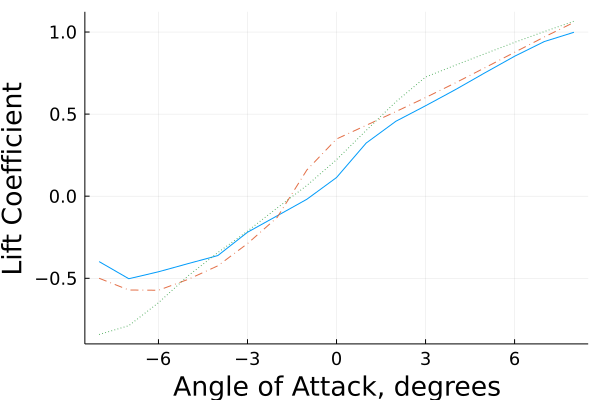
\includegraphics[width = .35\textwidth]{Plots/Figure13.png}}
	\subfloat[]{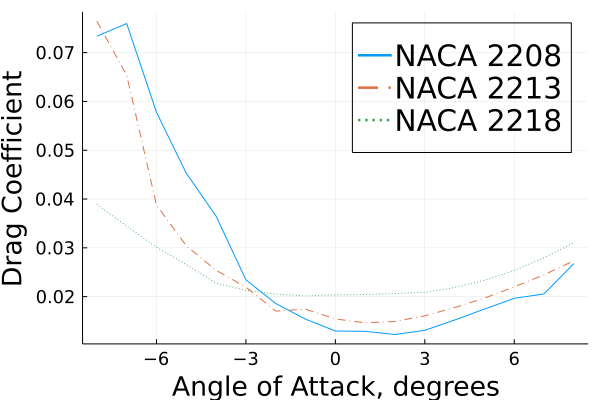
\includegraphics[width = .35\textwidth]{Plots/Figure14.png}}
	\caption{(a) Lift and (b) drag coefficients of NACA 4412 airfoils}
	\captionsetup{aboveskip=0pt,font=it}
	\label{afplot}
\end{figure}

\added[comment = {}]{After the airfoil was created, I lofted it over the APC 10x7 rotor used in the project, and evaluated the propeller's torque and power coefficients across a range of advance ratios with CCBlade.jl. Propellers in the optimization were compared at a specific advance ratio, $J=0.472$, which is explained later in this report and listed in the bottom entry of table} \eqref{ctab}. 

\added[comment = {}]{CCBlade.jl uses blade element momentum (BEM) theory}\footnote{More information about BEM theory can be found at \url{https://en.wikipedia.org/wiki/Blade_element_momentum_theory}} \added[comment = {}]{to calculate a propeller or turbine's behavior. BEM theory, which combines blade element theory and momentum theory, calculates the axial and tangential induction factors and the pitching angle, the angle between the free stream velocity and the tangential velocity of the propeller. After these three quantities are found, they are combined to find forces acting in all directions on the propeller}\cite{CCBlade}. 

\added[comment = {}]{I found the propeller's total torque and total moment from the torque output of the propeller's CCBlade.jl evaluation and from integration of the normal and tangential force data output by CCBlade.jl across the rotor blade using an integration function from the QuadGK.jl package. With the rotor blade's dimensions known, the moments and torque found by integrating with QuadGK.jl provided reasonable limits for use in the optimization.}

\subsection{Optimization}

\added[comment = {}]{I preformed two different optimizations in my propeller design. One optimization only maximized its efficiency, and another maximized efficiency while maintaining torque within 90\% of the original. These two optimizations converged to different propeller designs.} 

\added[comment = {}]{Propeller blade thickness in both designs was not allowed to increase or decrease by a factor of more than 2, and the propeller could not pitch more than} $90^{\circ}$ \added[comment = {}]{in either direction. The propeller's torque and normal and tangental moments did not exceed 110\% of the values calculated from the CCBlade.jl output when the original propeller was created. Equation} \eqref{Jequations} \added[comment = {}]{show how the advance ratio was calculated.} $v_{\infty}$ \added[comment = {}]{represents the free stream velocity,} $n$ is \added[comment = {}]{rotational velocity in revolutions per second, and} $D$ \added[comment = {}]{is the outer diameter.}

\begin{equation}
	\begin{aligned} 
	J & = \frac{v_{\infty}}{n D} \\
	& = \frac{12}{(\frac{6000}{60}) \times 0.254}
	\end{aligned}
	\label{Jequations}
\end{equation}

\added[comment = {}]{Table} \eqref{ctab} \added[comment = {}]{shows shared features and design variables of the propellers optimized. The advance ratio, $J$, is available from other variables already listed in the table by equation} \eqref{Jequations}. \added[comment = {}]{These values provided all the environmental and design variables I used.}

\begin{table}[H]
 \centering
 \begin{tabular}{| c | c | c | c |} \hline
 	 \textbf{parameter} & \textbf{default value} & \textbf{minimum value} & \textbf{maximum value} \\ \hline
	 chord length, & 100\% length & 50\% & 200\% \\ \hline
	 pitching angle, & $0^{\circ}$ & $-90^{\circ}$ & $90^{\circ}$ \\ \hline \hline
	 rotational velocity & \multicolumn{3}{c|}{6000 RPM} \\ \hline
	 blade count & 3 blades & \multicolumn{2}{c|}{2, 3, or 4}\\ \hline
	 hub-to-tip ratio & \multicolumn{3}{c|}{10\%} \\ \hline
	 air density & \multicolumn{3}{c|}{1.225 kg/$m^{3}$} \\ \hline
	 outer diameter & \multicolumn{3}{c|}{0.254 m (10 in.)} \\ \hline
	 velocity & \multicolumn{3}{c|}{12 m/s (26.84 mph)} \\ \hline
	 advance ratio & \multicolumn{3}{c|}{0.472} \\ \hline
 \end{tabular}
 \caption{Initial values and limits in propeller design}
 \label{ctab}
\end{table}

\subsubsection{\added[comment = {}]{No Minimum Torque}}

\added[comment = {}]{In both optimizations, I modified the chord length and pitching angle for propellers at the same advance ratio to find the most efficient one. The objective function, design variables, and constraints of the optimization without a minimum torque are displayed in equation} \eqref{optimization}, \added[comment = {}]{with the advance ratio $J=0.475$ calculated from equation} \eqref{Jequations}. 

\begin{equation}
	\begin{aligned}
		\mathrm{maximize:}& ~~ \eta ~ \text{at} ~ J = 0.475 \\
		\mathrm{with~respect~to:}& ~~ c & \multicolumn{1}{l}{$\theta$} \\
		\mathrm{subject~to:}& ~~ 50\% \leq c \leq 200\% & -90^{\circ} \leq \theta \leq 90^{\circ} \\
		& ~~ M_{n} \leq 1.1 M_{n0} & M_{t} \leq 1.1 M_{t0} \\
		& ~~ T \leq 1.1 T_{0} \\
	\end{aligned}
	\label{optimization}
\end{equation}

\deleted[comment = {}]{The objective function, equation} \eqref{1} \deleted[comment = {}]{was optimized using SNOW.jl.} \added[comment = {}]{SNOW.jl, developed by the FLOW Lab, finds either the maximum or minimum of a function.} The code \added[comment = {}]{used to design the propeller} was \deleted[comment = {}]{designed} \added[comment = {}]{prepared} so that SNOW.jl found the maximum \added[comment = {}]{of the objective function} by finding the minimum of its negative. This is similar to the technique \added[comment = {}]{and sign convention described} \deleted[comment = {}]{used} by Martins and Ning in \deleted[comment = {}]{page 10 of} \emph{Engineering Design Optimization}\cite{EngDesOpt}. \added[comment = {}]{SNOW.jl can also use fixed environmental variables and set limits or constraints on design variables to contain the domain of possible solutions that can be optimized. The program written for this project used both of these inputs to obtain the desired solutions, so SNOW.jl was a very useful tool.}

\added[comment = {}]{One discovery gained from these findings is that blades with smaller chord length make more efficient propellers. This finding is related to the rotor solidity, described in equation} \eqref{solid}. \added[comment = {}]{The optimization using SNOW.jl found the minimum chord length as the most efficient each time. Another evidence that increasing solidity decreases efficiency can be observed in figure} \eqref{efftqtab} \added[comment = {}]{in the conclusion. The rotor solidity increased proportionally to the blade count. As it increased, the efficiency at each advance ratio decreased.}

\begin{equation}
	\begin{aligned}
	\sigma & = \frac{c}{s} \\
	& = \frac{c n_{b}}{2 \pi \sqrt{\frac{r_{h}^{2}+r_{t}^{2}}{2}}}
\end{aligned}
\label{solid}
\end{equation}

\added[comment = {}]{All of the propellers optimized had the lowest chord length allowed by the program used. Equation} \eqref{solid} \added[comment = {}]{shows that reducing the chord length,} $c$, \added[comment = {}]{or the blade count,} $n_{b}$, \added[comment = {}]{reduces the solidity,} $\sigma$. \added[comment = {}]{The finding that lower solidity leads to greater efficiency seems reasonable, because wind turbines with long, thin blades, designed to efficiently harvest wind from the environment, have very low solidity according to this equation. This finding about propeller blades with less solidity being more efficient also agrees with Saraf, Nouli, Ravalet, and Bakir's findings}\cite{AxFlFan}.

\added[comment = {}]{With this information, I decided to find what the optimal chord length actually was. Figure} \eqref{mag} \added[comment = {}]{shows what happened when I removed the original  50\% lower limit of the optimizer and instead set it to 1\% in the function argument. SNOW.jl found a propeller that was much more efficient, and had exactly 1\% of the original chord length.}

\begin{figure}[H]
\centering
 	\subfloat{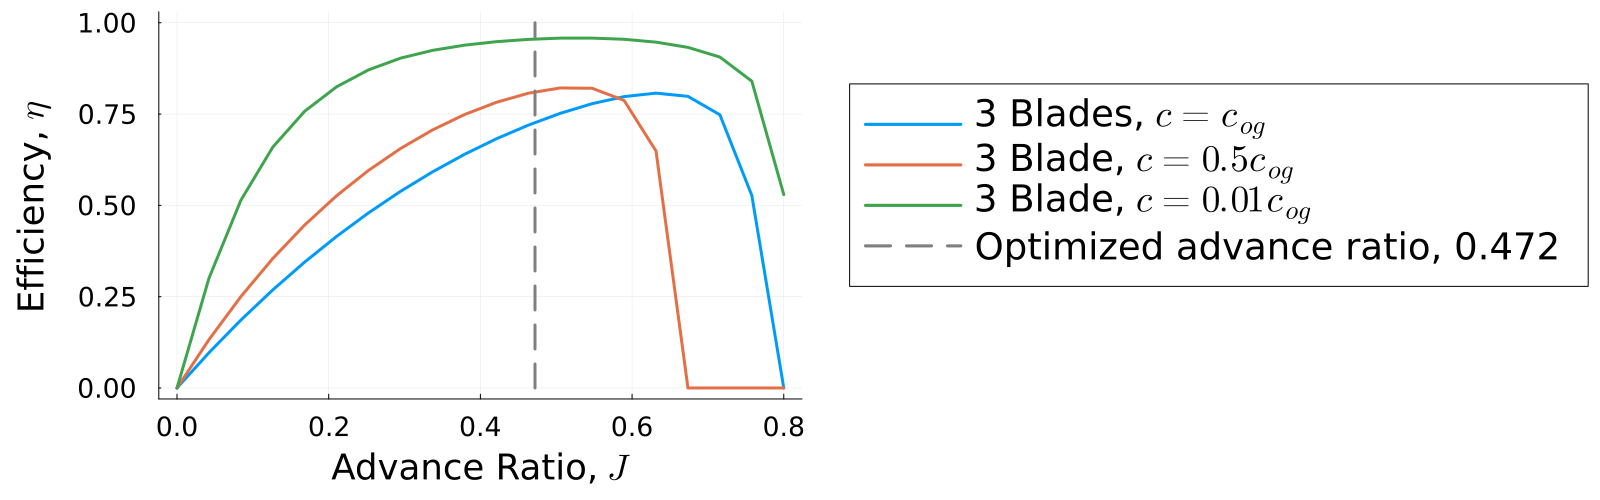
\includegraphics[width = .70\textwidth]{Plots/Figure_6.png}}
	
	\caption{Comparison of propellers with different cord lengths}
	\captionsetup{aboveskip=0pt,font=it}
	\label{mag}
\end{figure}

\added[comment = {}]{A propellor with a chord length that much smaller is unrealistic to actually use, though, because it would produce hardly any thrust compared to the original propeller. One APC 10x7 propeller found on the internet had a 1.02 cm hub thickness to start with}\footnote{This propeller was found at \url{https://www.apcprop.com/product/10x7e/}.}, \added[comment = {}]{and lowering the chord to 1\% would decrease that to 102{\textmu}m. It appears that even in extreme cases, decreasing chord length always increases propeller efficiency even when it is most likely no longer desired.}

\added[comment = {}]{One significant problem with the first optimization is that a propeller's efficiency can be obtained as a function of its advance ratio, thrust coefficient, and power coefficient. The equation for efficiency is described by Andrew Ning in \emph{Computational Aerodynamics}}\cite{ComAer}, \added[comment = {}]{using the relations in equation} \eqref{etqeq}.

\begin{equation}
	\begin{aligned}
	\eta & = J \frac{C_{T}}{C_{P}} \\
	& = \frac{T V_{\infty}}{T V_{\infty} + \frac{1}{2} \dot{m} (V_{w} - V_{\infty})^{2}}
	\end{aligned}
\label{etqeq}
\end{equation}

\added[comment = {}]{Ning also wrote that when thrust is increased for a propeller, it comes at the expense of decreased efficiency}\cite{ComAer}. \added[comment = {}]{Conversely, a propeller optimization that maximizes efficiency will decrease its thrust coefficient. The torque and moments output by the optimized propellers did not even come near the limits put in place by the original propeller. For example, the original propeller blades experienced a normal moment of $3.753 \times 10^{6}N \times m$, but the optimized propeller with the same blade count only experienced $3.808 \times 10^{5} N \times m$.}

\added[comment = {}]{When I kept} $J$ \added[comment = {}]{constant in this research, inspection of figure} \eqref{efftqtab} \added[comment = {}]{in the results section reveals that the optimizer maximized equation} \eqref{optimization} \added[comment = {}]{by minimizing} $C_{P}$, \added[comment = {}]{which is equal to} $C_{Q}$ \added[comment = {}]{multiplied by} $2 \pi$. \added[comment = {}]{The torque coefficient} $C_{Q}$ \added[comment = {}]{is significantly lower for each propeller. While the thrust coefficient} $C_{T}$ \added[comment = {}]{did not decrease by as much as} $C_{Q}$, \added[comment = {}]{it is still much lower than before. Although more efficient, the newly optimized propeller outputs much less power and may be better suited for an entirely different function than the one it started with.}

\added[comment = {}]{Another discovery made in the optimization without a minimum torque requirement was that this propeller was most efficient with negative blade pitching angle. To investigate this result further, I ran another simulation with the Julia code I had written to see what happened to this blade pitching angle when the propeller was increase back to its original chord length. The plot in figure} \eqref{same} \added[comment = {}]{shows the original propeller compared to the optimized propeller, shown in figure} \eqref{efftqtab} \added[comment = {}]{and discussed in the results section, and a propeller with the optimized pitching angle but the same chord magnification as the original propeller.} 

\begin{figure}[H]
\centering
 	\subfloat{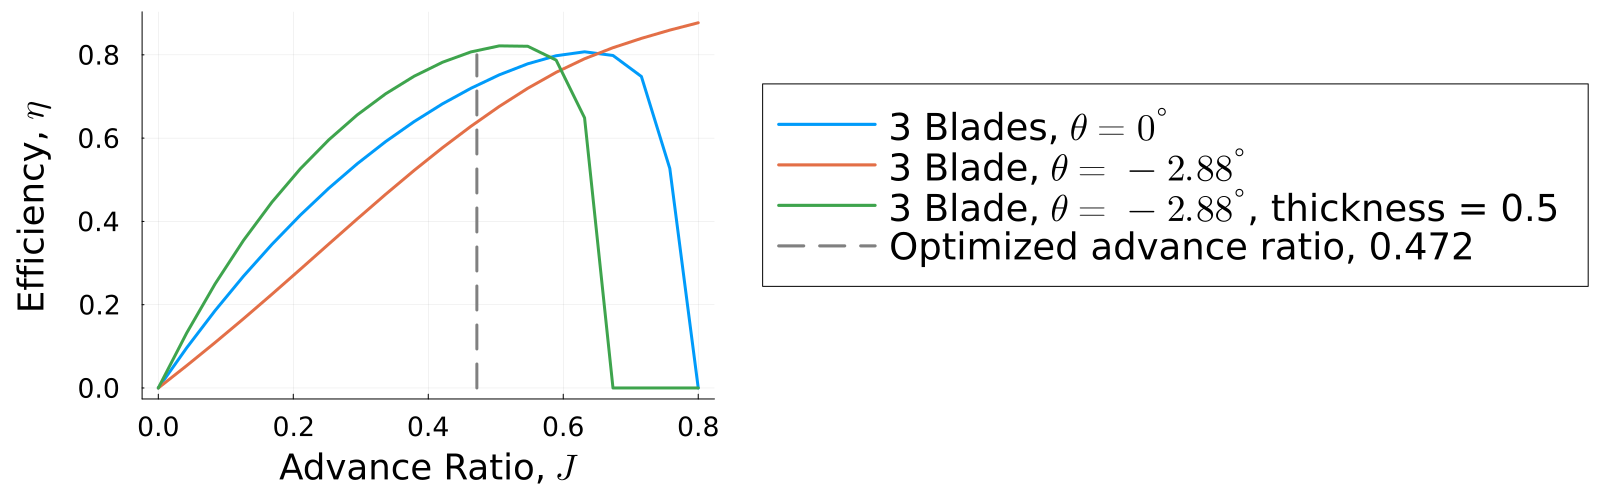
\includegraphics[width = .70\textwidth]{Plots/Figure_5.png}}
	
	\caption{Comparison of identical propellers at different pitching angles to optimized propeller}
	\captionsetup{aboveskip=0pt,font=it}
	\label{same}
\end{figure}

\added[comment = {}]{The different curves plotted in figure} \eqref{same} \added[comment = {}]{show that the propeller only became more efficient at the $-2.88^{\circ}$ pitching angle when its chord length was also reduced significantly. Otherwise, it became less efficient at the advance ratio measured but more efficient at higher advance ratios. This showed that rotors with different chord length are better suited for different rotational velocities and free stream velocities, discussed in equation} \eqref{Jequations}. \added[comment = {}]{The optimization described previously increased the efficiency, but only for much thinner propeller blades.}

\added[comment = {}]{Table} \eqref{resultstab} \added[comment = {}]{in the results section shows that although the optimal pitching angles were very similar for all three different blade counts, they became minutely more negative as the blade count increased. This further decrease in the already negative pitching angle could be at least partially explained by the airfoil polars shown in figure} \eqref{afplot}. \added[comment = {}]{Increasing the pitching angle slightly above} $-3^{\circ}$ \added[comment = {}]{would make its lift coefficient higher and its drag coefficient slightly lower. Figure} \eqref{afplot}, \added[comment = {}]{from airfoil analysis conducted earlier in the semester, shows that angles of attack near} $-3^{\circ}$ \added[comment = {}]{for the NACA 4412 airfoil used in this design correspond to a very low drag coefficient.}

\added[comment = {}]{Changing the pitching angle of this propeller would change the forces and efficiency produced by a propeller with a blade count of 2 differently than propellers with blade counts of 3 or 4, because the wake instability created by each propeller blade affects the other blades}\cite{bceff}. \added[comment = {}]{This change in blade-to-blade interactions is one reason why the curves in figure} \eqref{efftqtab} \added[comment = {}]{are shaped differently from each other, even though they are optimizations of propellers with the same airfoil and rotor profiles.}

\subsubsection{Minimum Torque Added}

\added[comment = {}]{To prevent the optimizer from sacrificing thrust for efficiency, I provided a minimum torque as a parameter along with the maximums shown below the objective function in equation} \eqref{optimization}. \added[comment = {}]{I used this additional constraint to find the pitching angle and chord magnification that would provide the maximum efficiency while still maintaining some required thrust or being powered by the same motor. This way, the optimizer did not reduce the propeller to its minimum possible chord length in every case as it did in this optimization.}

\added[comment = {}]{I combated the problem of the optimizer maximizing efficiency by minimizing the thrust coefficient as shown in equation} \eqref{etqeq} \added[comment = {}]{by adding a minimum torque requirement to the optimization. The updated requirements matrix with the torque requirement changed from equation} \eqref{optimization} \added[comment = {}]{is shown below, in equation} \eqref{newopt}:

\begin{equation}
	\begin{aligned}
		\mathrm{maximize:}& ~~ \eta ~ \text{at} ~ J = 0.475 \\
		\mathrm{with~respect~to:}& ~~ c & \multicolumn{1}{l}{$\theta$} \\
		\mathrm{subject~to:}& ~~ 50\% \leq c \leq 200\% & -90^{\circ} \leq \theta \leq 90^{\circ} \\
		& ~~ M_{n} \leq 1.1 M_{n0} & M_{t} \leq 1.1 M_{t0} \\
		& ~~ 0.9 T_{0} \leq T \leq 1.1 T_{0} \\
	\end{aligned}
	\label{newopt}
\end{equation}

\added[comment = {}]{The torque coefficient} $C_{Q}$ \added[comment = {}]{and power coefficient} $C_{P}$ \added[comment = {}]{are related by a factor of} $2 \pi$, \added[comment = {}]{so keeping the propeller torque within 90\% of the original would also maintain 90\% of the original power output, or} $P \geq 0.9 P_{0}$. \added[comment = {}]{The minimum torque requirement ensures that SNOW.jl will not give the unwanted results in figure} \eqref{mag} \added[comment = {}]{and figure} \eqref{same}

\section{\added[comment = {}]{Results and} Discussion}

\deleted[comment = {}]{The propeller was checked at blade counts of 1, 2, and 3. These results found that for all three blade counds, the optimal propellor was as thin as possible, with a smal negative angle of attack. The finding about thinner rotor blades being more efficient agrees with Saraf, Nouli, Ravalet, and Bakir's findings, but the negative rotation angle was a surprise at first.}

\deleted[comment = {}]{One lesson learned from this optimization is that the user should be careful what is optimized for, because the computer will optimize exactly what it is told, even if that is not what the user actually wants. An optimization that is written incorrectly or has unseen loopholes can not only give a misleading answer but also waste a lot of time. In the case of this optimization, I think other constraints could have been added to the optimization.}

\added[comment = {}]{Although the propeller's profile remained the same throughout the first optimization, the chord length decreased for all blade counts. Changing the pitching angle rotated the propeller blade, and changing the chord magnified the size of its entire profile uniformly along its entire length. Rotor and airfoil themselves retained the same NACA and APC identification numbers throughout the optimization.}

\subsection{\deleted[comment = {}]{Efficiency Equation}}

\added[comment = {}]{Figure} \eqref{efftqtab} \added[comment = {}]{demonstrates that while the optimized design increased the efficiency of even the propeller with the higher blade count above the propeller pre-optimization, it dramatically decreased the thrust and torque coefficients. The efficiency at higher advance ratios also went to zero more quickly, so the range of advance ratios over which the propeller maintained high efficiency was smaller. Maximizing the propeller efficiency at a single advance ratio by only changing the chord length and pitching angle requires other propeller performance measures to be sacrificed.}

\begin{figure}[H]
\centering
 	\subfloat[]{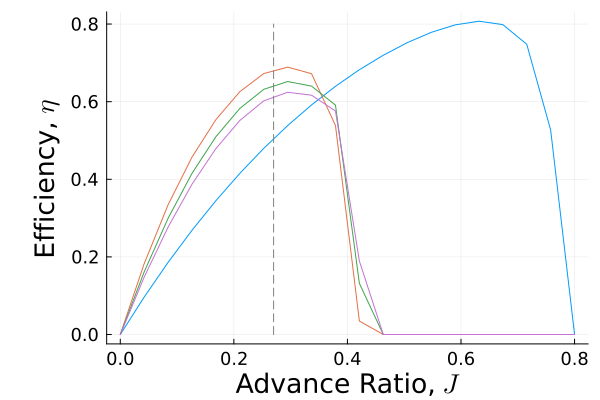
\includegraphics[width = .35\textwidth]{Plots/Figure_1.png}}
	\subfloat[]{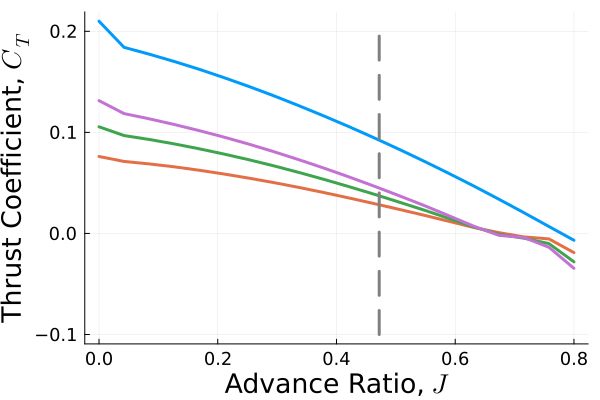
\includegraphics[width = .35\textwidth]{Plots/Figure_2.png}}

	\subfloat[]{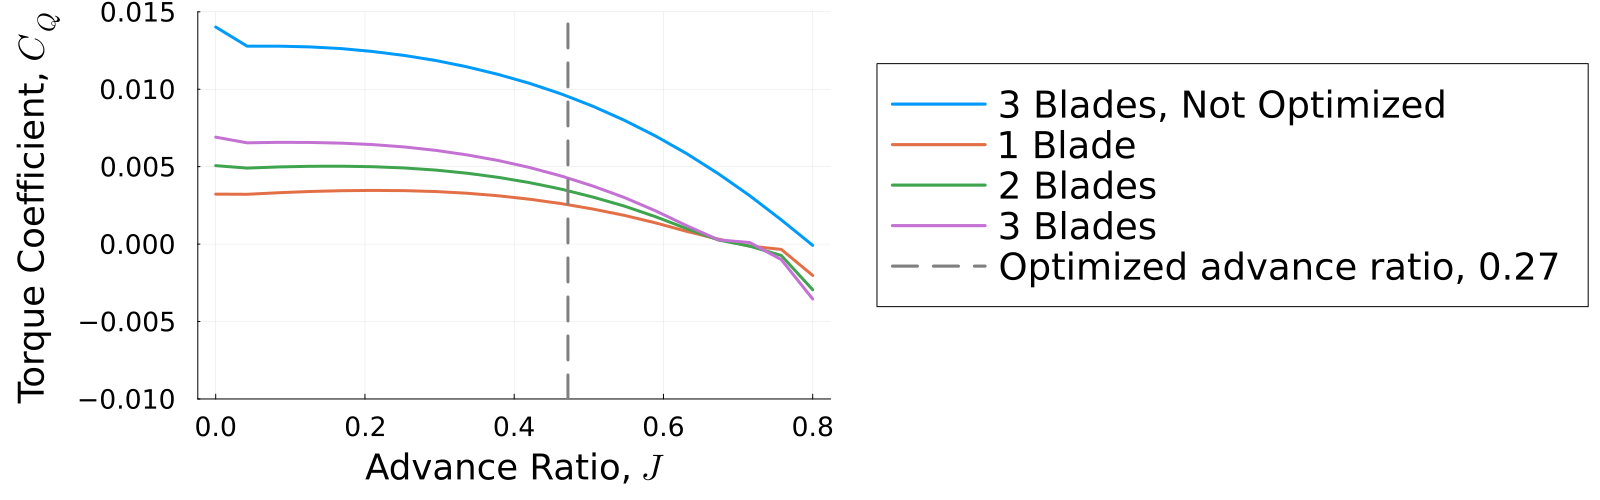
\includegraphics[width = .70\textwidth]{Plots/Figure_3.png}}\hspace{1em}
	\caption{(a) Efficiency, (b) thrust coefficient, and (c) torque coefficient compared at different advance ratios}
	\captionsetup{aboveskip=0pt,font=it}
	\label{efftqtab}
\end{figure}

\added[comment = {}]{Table} \eqref{resultstab} \added[comment = {}]{shows the optimal pitching angles and chord magnifications found by SNOW.jl for each different propeller blade count. At the conditions listed in table} \eqref{ctab}, \added[comment = {}]{the same optimal chord length magnification was found, and the optimal pitching angle was less than} $-3^{\circ}$ \added[comment = {}]{for each propeller. These results prove a few things about the propeller designed.}

\begin{table}[H]
 \centering
 \begin{tabular}{| c | c | c |} \hline
 	 \textbf{blade count} & \textbf{chord length magnification} & \textbf{pitching angle} \\ \hline
  	 3 (Default) & 1.0 & $0^{\circ}$ \\ \hline
  	 2 & 0.500 & $-2.70^{\circ}$ \\ \hline
  	 3 & 0.500 & $-2.88^{\circ}$ \\ \hline
  	 4 & 0.500 & $-2.94^{\circ}$ \\ \hline
	 3 ($P \geq 0.9 P_{0}$) & 0.532 & $2.96^{\circ}$ \\ \hline
 \end{tabular}
 \caption{Optimized chord magnification and pitching angles for different blade counts}
 \label{resultstab}
\end{table}

\added[comment = {}]{The plots in figure} \eqref{perspow} \added[comment = {}]{show two results of the new design, with the minimum thrust requirement. First, the propeller efficiency increases at the measured advance ratio, but not by quite as much as the propeller without the minimum power constraint. Second, it is even more efficient at higher advance ratios. This optimized propeller's final chord length was still decreased to 53.2\% of its original chord length, which was near although not quite at the 50\% lower limit given to SNOW.jl. Unlike the propellers optimized previously, though, this optimized propeller's pitching angle was positive,} $2.96^{\circ}$.

\begin{figure}[H]
\centering
 	\subfloat[]{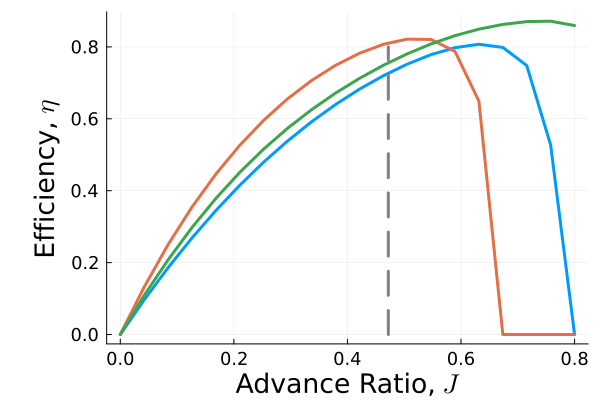
\includegraphics[width = .35\textwidth]{Plots/Figure_7.png}}
	\subfloat[]{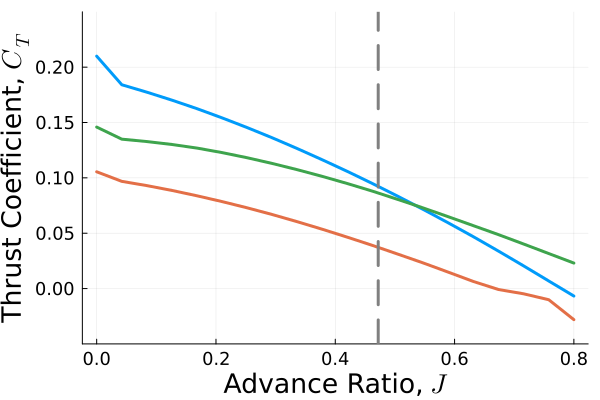
\includegraphics[width = .35\textwidth]{Plots/Figure_8.png}}

	\subfloat[]{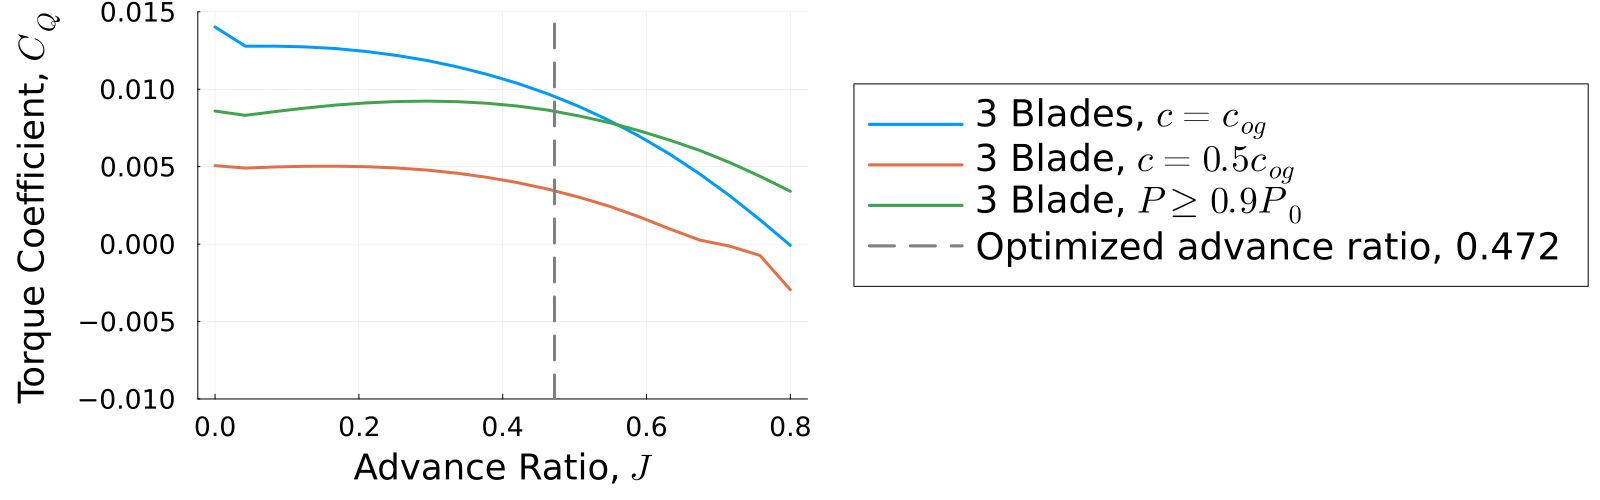
\includegraphics[width = .70\textwidth]{Plots/Figure_9.png}}\hspace{1em}
	\caption{Efficiency (a), thrust coefficient (b), and torque coefficient (c) compared between different optimizations}
	\captionsetup{aboveskip=0pt,font=it}
	\label{perspow}
\end{figure}

\deleted[comment = {}]{One problem with this optimization is that a rotor's efficiency is available as a fucntion of the advance ratio, the thrust coefficient, and the power coefficient. The equation for efficiency is described by Andrew Ning in \emph{Computational Aerodynamics}, page 200 using the relation below, equation} \eqref{d}

\begin{equation}
\begin{aligned}
	\eta = J \frac{C_{T}}{C_{P}}
\end{aligned}
\label{d}
\end{equation}

\deleted[comment = {}]{With J kept constant, as it was in this research, this equation can be maximized in either by maximizing} $C_{T}$ \deleted[comment = {}]{or by minimizing} $C_{P}$, \deleted[comment = {}]{which is equal to} $C_{Q}$ \deleted[comment = {}]{multiplied by} $2 \pi$ \deleted[comment = {}]{Inspection of figure} \eqref{efftqtab} \deleted[comment = {}]{reveals that the optimizer did the latter. The torque coefficient} $C_{Q}$ \deleted[comment = {}]{is significantly lower for each rotor. While the thrust coefficient} $C_{T}$ \deleted[comment = {}]{did not decrease by as much as} $C_{Q}$, \deleted[comment = {}]{it is still much lower than before. Although more efficient, the newly optimized propellor has a much lower solidity and is better suited for a different environment.}

\subsection{\deleted[comment = {}]{Angle of Rotation}}

\deleted[comment = {}]{The optimal angles of rotation were between} $-2.74^{\circ}$ \deleted[comment = {}]{and} $-2.94^{\circ}$ \deleted[comment = {}]{, as shown in table} \eqref{c}. \deleted[comment = {}]{These negative angles of rotation were surprising at firs, because angles near} $0^{\circ}$ \deleted[comment = {}]{were expected to be the most efficient. Figure} \eqref{e}, \deleted[comment = {}]{from airfoil analysis conducted earlier in the semester, shows that} $0^{\circ}$ \deleted[comment = {}]{angle of attack did not necessarily correspond to the lower lift and drag coefficients for the NACA 4412 airfoil used in this design. Although that finding was for more simple analysis of an airfoil, it was concluded that a negative angle of rotation was possible.}

\begin{figure}[H]
\centering
 	\subfloat[Lift Coefficient]{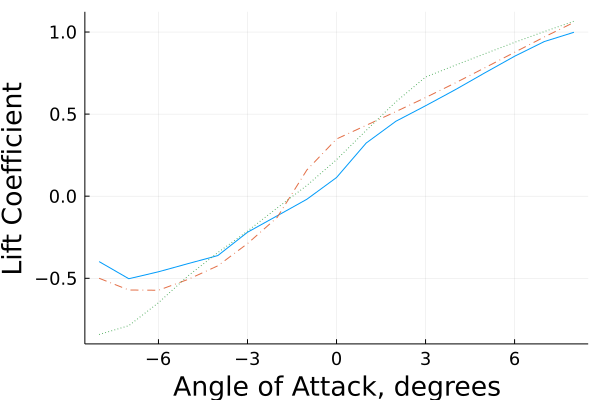
\includegraphics[width = .35\textwidth]{Plots/Figure13.png}}
	\subfloat[Drag Coefficient]{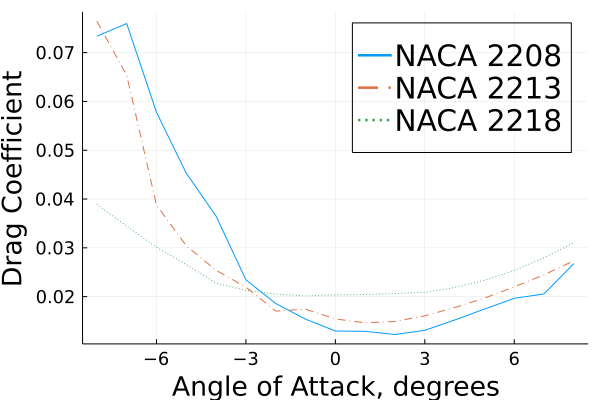
\includegraphics[width = .35\textwidth]{Plots/Figure14.png}}
	\caption{Lift and Drag Experienced by NACA 4412 Airfoils}
	\captionsetup{aboveskip=0pt,font=it}
	\caption*{These plots show how lift and drag change for an airfoil at different angles of attack.}
	\label{e}
\end{figure} 

\section{Conclusion}

\added[comment = {}]{In} this optimization, \added[comment = {}]{I used} \deleted[comment = {}]{combined} several Julia packages to find the optimal \added[comment = {}]{combination of chord length and pitching} angle \deleted[comment = {}]{of rotation and rotor chord length} for \deleted[comment = {}]{a rotor's} \added[comment = {}]{the maximum} efficiency \added[comment = {}]{of a propeller at a known advance ratio. I discovered that for the conditions listed in table \eqref{ctab}, the optimal propeller has 50\% its original chord length, which is the lower limit of the optimization, and a pitching angle between} $-2.70^{\circ}$ \added[comment = {}]{and} $-2.94^{\circ}$, d\added[comment = {}]{epending on the blade count.} \deleted[comment = {}]{I found that rotors with very small chord length at negative angles of rotation were the most efficient.}

\added[comment = {}]{After finding this result, I added a constraint to the minimum torque of the propeller, to ensure that it still transferred enough of its power to the air while being efficient. When I did this, I found the optimal pitching angle to be} $2.98^{\circ}$ \added[comment = {}]{and the optimal chord length magnification of 0.52. This proved that optimizations with just one additional constraint can produce very different results.}

\added[comment = {}]{Future work could investigate other possible constraints to place on this optimization, or change the constraints already present. Propellers can operate at many different advance ratios. Other optimizations could vary other aspects of the propeller. For example, the rotor length could be optimized while maintaining a maximum power output, or the shape of the airfoil could be changed entirely or even lofted through different shapes. The rotor could also be modified to an optimal shape. As long as the user understands well the constraints that must be met, optimizations have immense possibilities.} \deleted[comment = {}]{Other optimizations could be performed by simple editing of the code used in this research to find which other rotors perform best in other applications or environments.}

\added[comment = {}]{Performing an optimization aided by computers allowed me to explore a broader design space as new ideas were rapidly generated that had not been considered before.}


\section{Acknowledgements}

\deleted[comment = {}]{The author would like to thank} Adam, \deleted[comment = {}]{Cardoza} \added[comment = {}]{thank you} for mentoring \added[comment = {}]{me} \deleted[comment = {}]{him} in learning the codes used in the FLOW Lab, directing \deleted[comment = {}]{his} \added[comment = {}]{my} research, and helping \added[comment = {}]{me} \deleted[comment = {}]{him} through questions and challenges that \deleted[comment = {}]{he} \added[comment = {}]{I} encountered during this work.



\bibliography{Final_Report}

\end{document}